\subsection{Brightness}

The alteration under analysis now is the brightness, presented in \Fig~\ref{fig:acc_br_wu}.

It is evident from \Fig~\ref{fig:br_acc_wu_bnn} that the BNN exhibits good robustness for increasing brightness values. \Fig~\ref{fig:brightness_ann} demonstrates that the standard NN is not significantly affected by the alteration, as the accuracy remains around the nominal conditions without a substantial change.

\begin{figure}[h]
	\centering
	\begin{subfigure}{.5\textwidth}
		\centering
		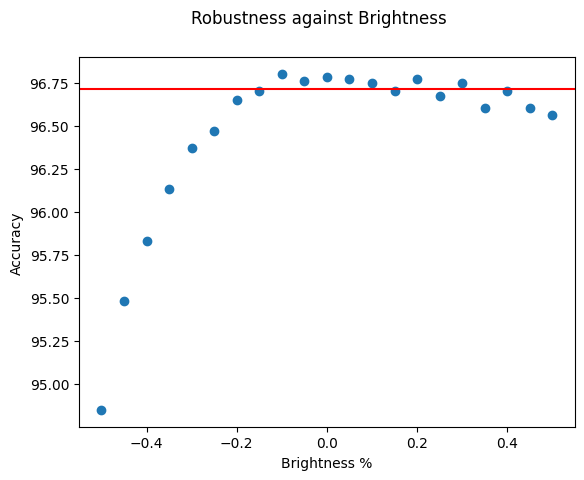
\includegraphics[width=0.8\linewidth]{ImageFiles/EvalBNN/BR/WU/acc}
		\caption{BNN}
		\label{fig:br_acc_wu_bnn}
	\end{subfigure}%
	\begin{subfigure}{.5\textwidth}
		\centering
		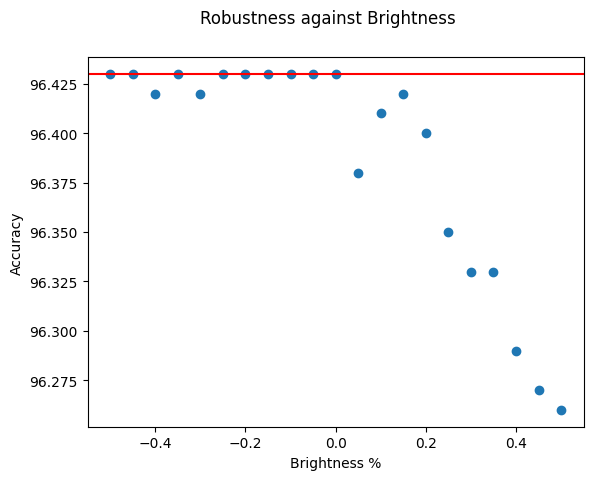
\includegraphics[width=0.8\linewidth]{ImageFiles/EvalANN/brightness_ann}
		\caption{Standard NN}
		\label{fig:brightness_ann}
	\end{subfigure}
	\caption{Accuracy trend for blur alteration}
	\label{fig:acc_br_wu}
\end{figure}

When computing robustness, the results are $0.9988$ for the BNN and $0.0.9998$ for the standard NN, demonstrating a similar robustness. These values are close to $1$, which suggests a good robustness from both the networks.

The aleatoric uncertainty, as shown in \Fig~\ref{fig:br_aleatoric}, follows a trend that aligns with the accuracy trend. The network exhibits higher uncertainty at lower alteration levels, where there was also a decrease in accuracy. 

\Fig~\ref{fig:br_epistemic} illustrates the trend of the epistemic uncertainty, which appears to oscillate but not significantly. This behavior may become clearer when using uncertainty in the classification.

\begin{figure}[h]
	\centering
	\begin{subfigure}{.5\textwidth}
		\centering
		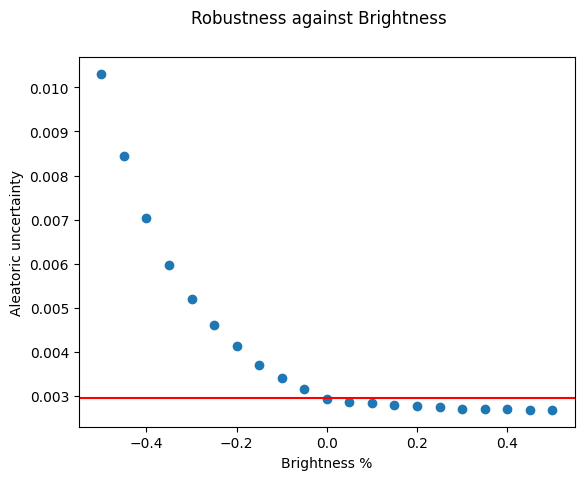
\includegraphics[width=0.8\linewidth]{ImageFiles/EvalBNN/BR/aleatoric}
		\caption{Aleatoric uncertainty}
		\label{fig:br_aleatoric}
	\end{subfigure}%
	\begin{subfigure}{.5\textwidth}
		\centering
		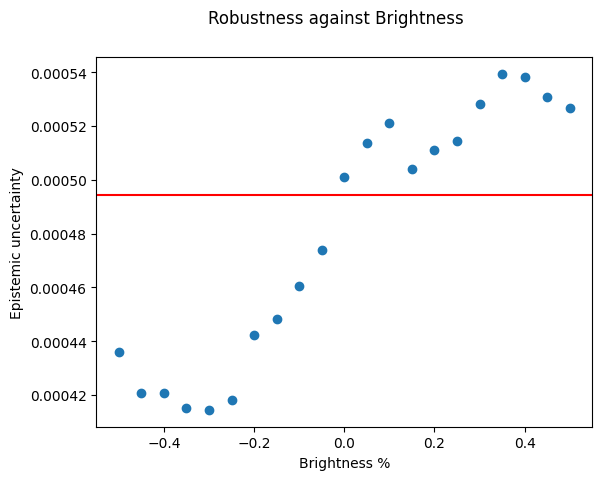
\includegraphics[width=0.8\linewidth]{ImageFiles/EvalBNN/BR/epistemic}
		\caption{Epistemic uncertainty}
		\label{fig:br_epistemic}
	\end{subfigure}
	\caption{Uncertainty trend for brightness alteration}
	\label{fig:br_uncertainty}
\end{figure}

\vspace{0.3cm}
\textbf{Classification using aleatoric uncertainty}
\vspace{0.1cm}

When utilizing aleatoric uncertainty in the classification, the accuracy, \Fig~\ref{fig:br_au_acc}, increases substantially, reaching even higher values for low brightness percentages. However, there is always the trade-off of the unknown ratio, which is high for negative percentages, as shown in \Fig~\ref{fig:br_au_unkn}. In this particular case, the effectiveness metric, \Fig~\ref{fig:br_au_eff}, provides meaningful information. It follows the trend of the accuracy without uncertainty, demonstrating that the metric is capable of revealing the network weaknesses. Using this aleatoric uncertainty in this case has the effect of converting incorrect predictions into unknown predictions, but the ratio still follows the original trend.

\begin{figure}[h]
	\centering
	\begin{subfigure}{.33\textwidth}
		\centering
		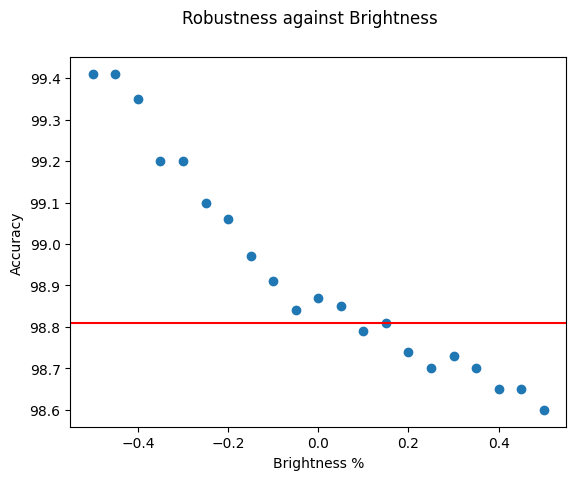
\includegraphics[width=0.9\linewidth]{ImageFiles/EvalBNN/BR/AU/acc}
		\caption{Accuracy using aleatoric \\ uncertainty}
		\label{fig:br_au_acc}
	\end{subfigure}%
	\begin{subfigure}{.33\textwidth}
		\centering
		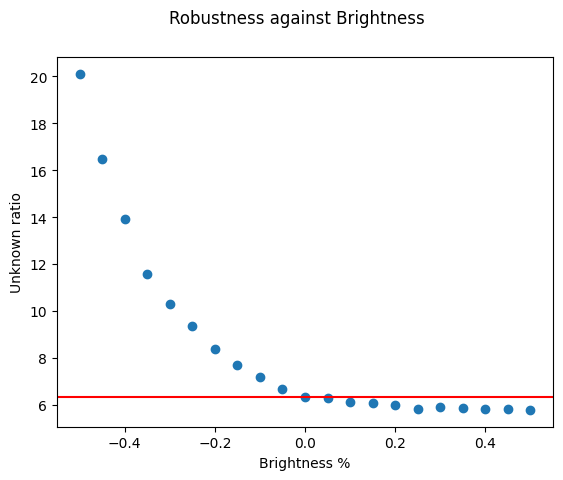
\includegraphics[width=0.9\linewidth]{ImageFiles/EvalBNN/BR/AU/unkn}
		\caption{Unknown ratio using aleatoric uncertainty}
		\label{fig:br_au_unkn}
	\end{subfigure}%
	\begin{subfigure}{.33\textwidth}
		\centering
		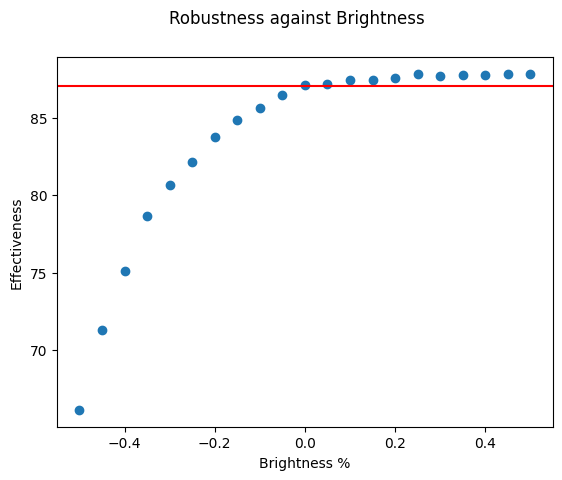
\includegraphics[width=0.9\linewidth]{ImageFiles/EvalBNN/BR/AU/eff}
		\caption{Effectiveness using aleatoric uncertainty}
		\label{fig:br_au_eff}
	\end{subfigure}
	\caption{Robustness graph for brightness when aleatoric uncertainty is employed in the classification}
	\label{fig:br_au}
\end{figure}

\Tab~\ref{table:rob_br_au} offers a summary of the robustness metrics resulting from this evaluation. It is possible to note reflect the observations made regarding the unknown ratio, especially by the augmented robustness.

\begin{table}[h]
	\centering
	\begin{tabular}{|| l | l ||} 
		\hline
		\textbf{Parameter} & \textbf{Value} \\
		\hline
		\hline
		$rob_{Brightness}$ & $0.9997$ \\
		$robInd_{Brightness}$ & $0.9890$ \\
		$robAug_{Brightness}$ & $0.9813$ \\	
		\hline
	\end{tabular}	
	\caption{Robustness metrics for the brightness when the aleatoric uncertainty is employed}
	\label{table:rob_br_au}
\end{table}

This analysis confirms again that the network can successfully identify situations of uncertainty. However, it also indicates that the network tends to be pessimistic, discarding more predictions than necessary.

\vspace{0.3cm}
\textbf{Classification using epistemic uncertainty}
\vspace{0.1cm}

Using the epistemic it is possible to achieve better performance in terms of unknown in this case, as shown in \Fig~\ref{fig:br_eu}. However, the accuracy has the same trend of the situation without use of uncertainty. In this particular scenario, the effectiveness, \Fig~\ref{fig:br_eu_eff}, benefits from it, as the accuracy was originally already high without the use of uncertainty.

In fact, \Fig~\ref{fig:br_eu_unkn} shows that the unknown ratio remains at low values even for negative percentages, indicating that using this uncertainty does not effectively recognize situations of uncertainty.

\begin{figure}[h]
	\centering
	\begin{subfigure}{.33\textwidth}
		\centering
		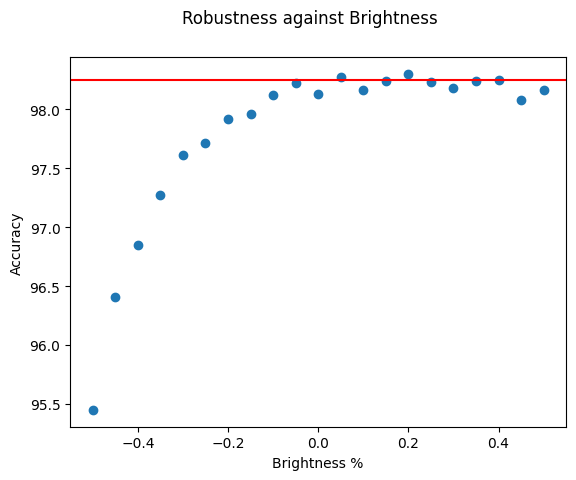
\includegraphics[width=0.9\linewidth]{ImageFiles/EvalBNN/BR/EU/acc}
		\caption{Accuracy using epistemic \\ uncertainty}
		\label{fig:br_eu_acc}
	\end{subfigure}%
	\begin{subfigure}{.33\textwidth}
		\centering
		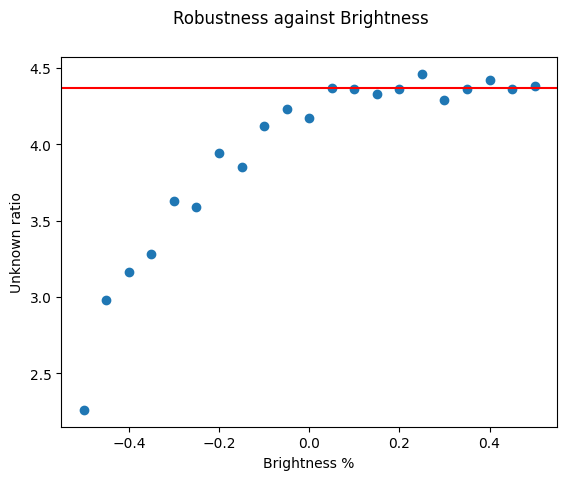
\includegraphics[width=0.9\linewidth]{ImageFiles/EvalBNN/BR/EU/unkn}
		\caption{Unknown ratio using \\ epistemic uncertainty}
		\label{fig:br_eu_unkn}
	\end{subfigure}%
	\begin{subfigure}{.33\textwidth}
		\centering
		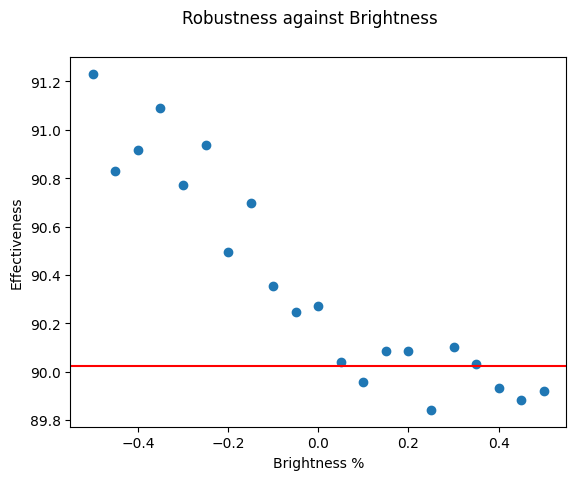
\includegraphics[width=0.9\linewidth]{ImageFiles/EvalBNN/BR/EU/eff}
		\caption{Effectiveness using \\ epistemic uncertainty}
		\label{fig:br_eu_eff}
	\end{subfigure}
	\caption{Robustness graph for brightness when epistemic uncertainty is employed in the classification}
	\label{fig:br_eu}
\end{figure}

\Tab~\ref{table:rob_br_eu} presents the robustness metrics. While they are still high, the $rob$ metric is slightly lower than in the previous case. However, the high $robInd$ value improves the performance in terms of $robAug$. It is important to note that high $robInd$ value can be misleading, as they could indicate the inability to identify uncertain situations. In the analyzed case, the outputs are equivalent to the situation when no uncertainty was used.

\begin{table}[h]
	\centering
	\begin{tabular}{|| l | l ||} 
		\hline
		\textbf{Parameter} & \textbf{Value} \\
		\hline
		\hline
		$rob_{Brightness}$ & $0.9979$ \\
		$robInd_{Brightness}$ & $0.9999$ \\
		$robAug_{Brightness}$ & $0.9999$ \\	
		\hline
	\end{tabular}	
	\caption{Robustness metrics for the brightness when the epistemic uncertainty is employed}
	\label{table:rob_br_eu}
\end{table}

\vspace{0.3cm}
\textbf{Classification using standard deviation}
\vspace{0.1cm}

The results using standard deviation, \Fig~\ref{fig:br_vu}, follows the same behavior obtained by the employment of aleatoric uncertainty. In this case, the system seems to be more pessimistic, as shown in \Fig~\ref{fig:br_vu_unkn}, with a positive improvement in terms of accuracy, \Fig~\ref{fig:br_vu_acc}. However, once again the effectiveness, \Fig~\ref{fig:br_vu_eff}, recaps both trends.

The results obtained using standard deviation, as shown in \Fig~\ref{fig:br_vu}, follow the same behavior as when employing aleatoric uncertainty. In this case, the system appears to be more pessimistic, as indicated in \Fig~\ref{fig:br_vu_unkn}, with a positive improvement in accuracy, as seen in \Fig~\ref{fig:br_vu_acc}. However, once again, the effectiveness metric, \Fig~\ref{fig:br_vu_eff}, summarizes the pessimistic behavior.

\begin{figure}[h]
	\centering
	\begin{subfigure}{.33\textwidth}
		\centering
		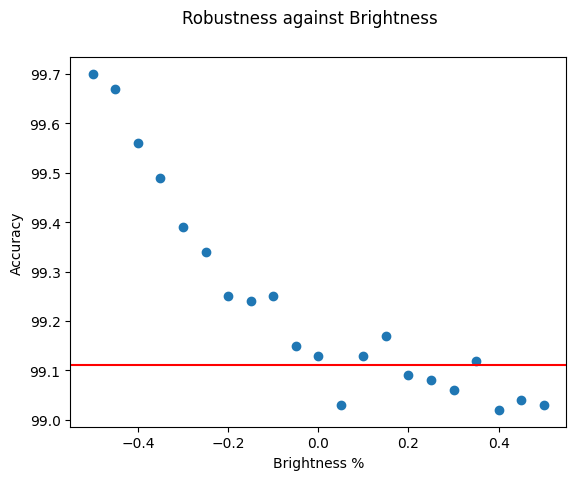
\includegraphics[width=0.9\linewidth]{ImageFiles/EvalBNN/BR/VU/acc}
		\caption{Accuracy using standard \\ deviation}
		\label{fig:br_vu_acc}
	\end{subfigure}%
	\begin{subfigure}{.33\textwidth}
		\centering
		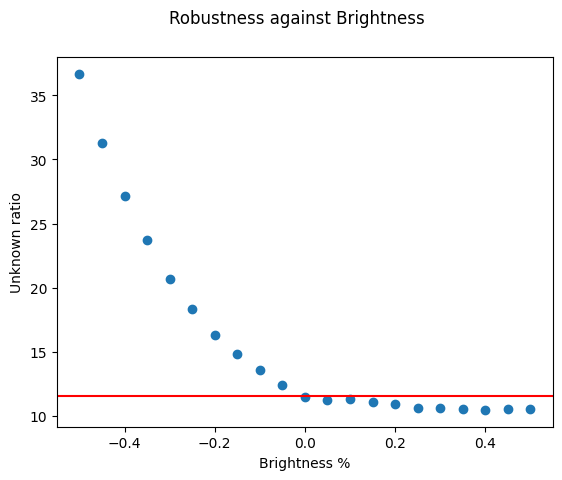
\includegraphics[width=0.9\linewidth]{ImageFiles/EvalBNN/BR/VU/unkn}
		\caption{Unknown ratio using \\ standard deviation}
		\label{fig:br_vu_unkn}
	\end{subfigure}%
	\begin{subfigure}{.33\textwidth}
		\centering
		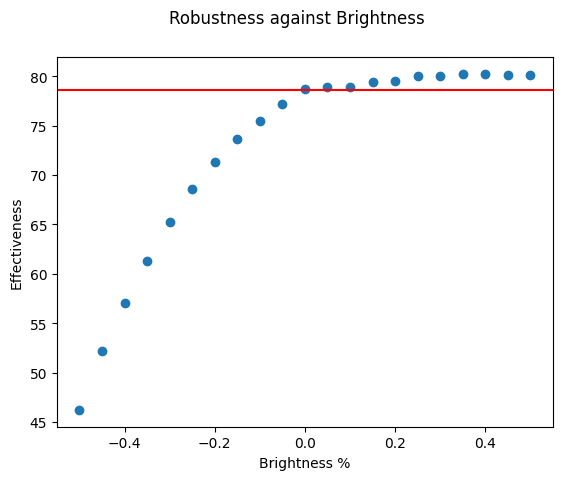
\includegraphics[width=0.9\linewidth]{ImageFiles/EvalBNN/BR/VU/eff}
		\caption{Effectiveness using standard deviation}
		\label{fig:br_vu_eff}
	\end{subfigure}
	\caption{Robustness graph for brightness when standard deviation is employed in the classification}
	\label{fig:br_vu}
\end{figure}

\Tab~\ref{table:rob_br_vu} provides the three robustness metrics. These values reflects the scenario when aleatoric uncertainty was employed.

\begin{table}[h]
	\centering
	\begin{tabular}{|| l | l ||} 
		\hline
		\textbf{Parameter} & \textbf{Value} \\
		\hline
		\hline
		$rob_{Brightness}$ & $0.9999$ \\
		$robInd_{Brightness}$ & $0.9754$ \\
		$robAug_{Brightness}$ & $0.9614$ \\	
		\hline
	\end{tabular}	
	\caption{Robustness metrics for the brightness when the standard deviation is employed}
	\label{table:rob_br_vu}
\end{table}

\vspace{0.3cm}
\textbf{Comparison}
\vspace{0.1cm}

\Tab~\ref{table:rob_br} summarizes the results obtained by the three classification methods. It is possible to conclude that network exhibits good inherent robustness to changes in brightness. The use of uncertainty highlighted the pessimistic behavior that the network can assume, especially with the standard deviation. This can be mitigated through an accurate tuning of the confidence level. On the other hand, epistemic uncertainty proved to be ineffective in this case, leading to a worse performance.

\begin{table}[h]
	\centering
	\begin{tabular}{|| l | l | l | l ||} 
		\hline
		\textbf{Parameter} & \textbf{Aleatoric} & \textbf{Epistemic} & \textbf{Standard deviation} \\
		\hline
		\hline
		$rob_{Brightness}$ & $0.9997$ & $0.9979$ & $0.9999$ \\
		$robInd_{Brightness}$ & $0.9890$ & $0.9999$ & $0.9754$ \\
		$robAug_{Brightness}$ & $0.9813$ & $0.9999$ & $0.9614$ \\	
		\hline
	\end{tabular}	
	\caption{Summary of the robustness metrics for the brightness alteration}
	\label{table:rob_br}
\end{table}